\begin{center}
\fbox{\fbox{\parbox{6.5in}{\centering
\begin{flushleft}
\hspace{5mm}
Lineaarne funktsioon $y=ax+b$ ja selle kordajad (tõus $a$ ja vabaliige $b$) kannavad endaga kaasas\\
\hspace{5mm} palju kasuliku informatsiooni. Lineaarse funktsiooniga saab näidata, kas tegemist on kasvava, või\\
\hspace{5mm} kahaneva protsessiga. Samuti võib selle funktsiooni tõusu järgi otsustada, kui kiiresti meil muutused\\
\hspace{5mm} mingis ''protsessis'' toimuvad.

\vspace{5mm}
\hspace{5mm}
\textbf{\underline{Mis määrab kasvamise ja kahanemise?}}

\vspace{2mm}
\hspace{5mm} Lineaarsefunktsiooni $y=ax+b$ korral määrab kasvamise ja kahanemise $x-i$ ees olev kordaja $a$.

\vspace{2mm}
\hspace{5mm}
Uurime näiteks kahte järgmist funktsiooni: $y=2x+5$ ning $y=-2x+5$.\\
\hspace{5mm}
Mõlemad funktsioonid näevad küll sarnased välja, kuid ühel on $x$-i ees $-2$ ja teisel $2$.\\
\hspace{5mm} Loome mõlema funktsiooni jaoks väärtuste tabelid ja joonestame nende graafikud.\\
\vspace{5mm}
\hspace{15mm} $y=2x+5$ tabel:\hspace{3mm}
\begin{tabular}{c|c|c}
     x & -1 & 1  \\
     \hline
     y & 3 & 7
\end{tabular}
\hspace{25mm} $y=-2x+5$ tabel: \hspace{3mm}
\begin{tabular}{c|c|c}
     x & -1 & 1\\
     \hline
     y & 7 & 3
\end{tabular}
\begin{center}
\begin{minipage}{7cm}
  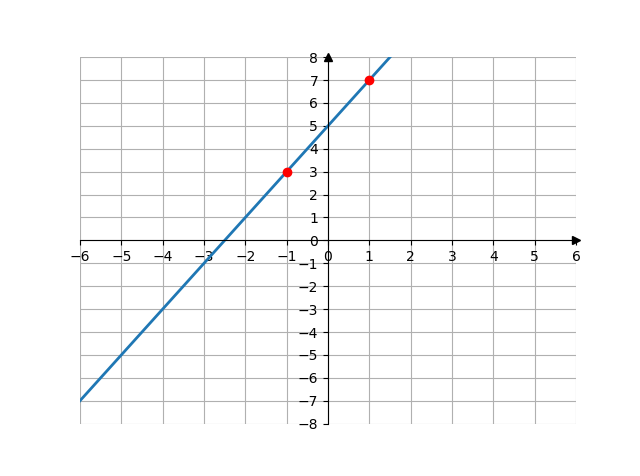
\includegraphics[width=7cm]{y=2x+5.png}
  \captionof{figure}{$y=2x+5$}
  \label{img3}
\end{minipage}
\hspace{.05\linewidth}
\begin{minipage}{.45\linewidth}
  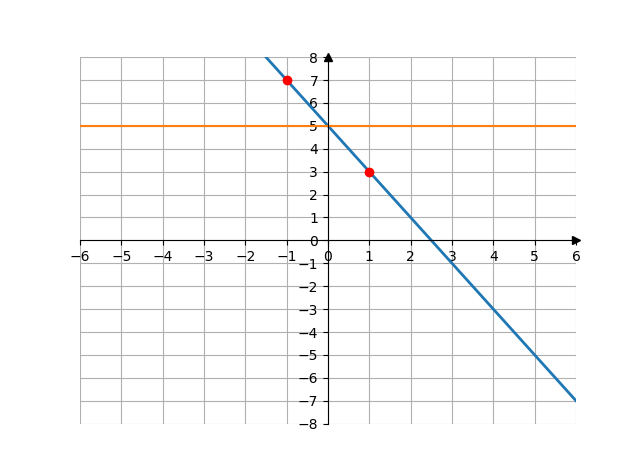
\includegraphics[width=7cm]{y=-2x+5.png}
  \captionof{figure}{$y=-2x+5$}
  \label{img4}
\end{minipage}
\end{center}

\hspace{5mm} Nagu jooniselt \ref{img3} näha, siis tõepoolest funktsiooni $y=2x+5$ korral toimub meil $x$ väärtuste\\ \hspace{5mm} suurenemisel ka $y$ väärtuste suurenemine. Küll aga $y=-2x+5$ korral (joonis \ref{img4}), kui $x$ suureneb,\\ \hspace{5mm} siis $y$ hoopis kahaneb. Seda erinevust võib tähele panna ka väärtuste tabelites:\\ \hspace{5mm} $y=2x+5$ tabelis on näha, et kui $x$ hüppab $-1$-lt $1$-le, siis $y$ hüppab $3$-lt $7$-le ($x$-i kasvades kasvab ka \\ \hspace{5mm} $y$). Aga $y=-2x+5$ tabeli korral, kui $x$ hüppab $-1$-lt $1$-le, siis $y$ hüppab hoopis $7$-lt $3$-le (ehk $x$-i\\ \hspace{5mm} kasvades muutub $y$ väiksemaks).\\ \hspace{5mm} Lisaks on joonisele \ref{img4} märgitud oranžiga ka funktsiooniga $y=0x+5$ määratud sirge. See on sarnane\\ \hspace{5mm} funktsiooniga $y=-2x+5$, kuid -2 asemel on 0. Näeme, et seal $x$-i kasvamisel $y$ ei muutu. See on\\ \hspace{5mm} sellepärast, et mistahes $x$-i valikul, jääb meil pealiige 0-ks.\\
\hspace{5mm} Seda saab näidata ka $y=0x+5$ väärtuste tabeliga:\\
\vspace{2mm}
\hspace{5mm}
\begin{tabular}{c|c|c|c|c|c}
     x & -2 & -1 & 0 & 1 & 2 \\
     \hline
     y & 5 & 5 & 5 & 5 & 5
\end{tabular}

\vspace{2mm}
\hspace{5mm}
Näeme, et sõltumata $x$-i valikust tuleb meil funktsiooni $y=0x+5$ väärtuseks alati 5, kuna  $x$-i\\ \hspace{5mm} ees on kordaja $0$ ja nende kahe arvu läbi korrutamisel tuleb tulemuseks alati 0. See aga vihjab selle,\\ \hspace{5mm} et muutusi sellise funktsiooni puhul ei toimu.\\
\vspace{2mm}
\hspace{5mm} Järeldused järgmisel lehel...
\end{flushleft}}}}
\end{center}


\newpage


\begin{center}
\fbox{\fbox{\parbox{6.5in}{\centering
\begin{flushleft}

\vspace{2mm}
\hspace{5mm}
Siit saamegi teha järgmised järeldused:\\
\vspace{2mm}
\hspace{5mm} Kui tõus $a$ on positiivne, ehk $a>0$, siis toimub KASVAMINE.\\
\vspace{2mm}
\hspace{5mm} Kui tõus $a$ on negatiivne, ehk $a<0$, siis toimub KAHANEMINE.\\
\vspace{2mm}
\hspace{5mm} Kui tõus $a=0$, siis mingeid muutusi EI TOIMU.\\
\vspace{5mm}
\hspace{5mm} Samuti tasuks mainida: \textbf{mida suurem tõus $a$ on, seda KIIREMINI toimuvad kasvamised\\ \hspace{5mm} või kahanemised.}

\end{flushleft}
}}}
\end{center}


\vspace{1cm}
\textbf{Märkmed}\\
\vspace{2mm}
\begin{mdframed}[style=graphpaper]
\vspace{14cm}
\end{mdframed}